\documentclass[11pt]{article}
\usepackage[spanish]{babel}
\usepackage{graphicx}
\graphicspath{ {./imagenes/} }

\title{Proyecto \#2: Programación paralela\\
Algoritmo de Dijkstra\\
\large Estructura de datos y algoritmos II}

\author{Cabello, Sofía
\and López, Ricardo
\and Núñez, Diego}

\begin{document}

\maketitle{}

\section{Algoritmo utilizado y su implementación }


Primero que nada, es importante aclarar que nos basamos en código encontrado en (Matloff, 2012) con algunas modificaciones, ya que se generaba una condición de carrera que será explicada más adelante.
\par 
¿Cómo correr el programa? El programa recibe dos parámetros desde la terminal, uno para indicar el número de nodos que tendrá el grafo aleatorio (llamado nv dentro del programa) y otro para indicar si se deben imprimir los resultados. Aunque esta última opción parece un poco extra o tonta, fue muy útil para las pruebas de rendimiento.
\par 
El programa comienza llenando la matriz de adyacencia del grafo. Como el programa crea grafos ponderados bidireccionales, no se ingresan valores negativos a la matriz. Primero se llena una mitad y después los valores son copiados a la otra, ya que la matriz debe ser simétrica.
\par 
Después, se inicializan los valores de un arreglo de nv espacios que indica si un nodo todavía no ha sido visitado. Al nodo 0 le corresponde el espacio 0 de este arreglo, al 1 el espacio 1 y así sucesivamente hasta nv-1. Cuando existe un valor de 1, entonces el nodo todavía no ha sido visitado. A este arreglo se le conoce como no notDone.
\par
Junto al arreglo anterior se inicializan los valores de otro arreglo llamado mind, que almacena las distancias mínimas almacenadas hasta el momento hacia cada nodo. Por defecto, estas distancias se inicializan con el valor de la arista que conecta directamente a cualquier nodo con el nodo 0. Además, este arreglo almacena datos de tipo usigned, ya que esta versión del algoritmo que no utiliza una cola de prioridad no funciona con pesos negativos. 
\par
Teniendo todo listo comienza el algoritmo en sí. Se encuentra el constructor parallel, lo que significa que a partir de este punto se utilizarán varios hilos. Primero, se inicializan tres variables, step, mymv y mymd. La primera variable indica que nodo se está revisando en un momento. Cada nodo es revisado una vez, por esta razón step va desde 0 hasta nv-1. La segunda y la tercera sirven para almacenar de manera local para los hilos cual es el nodo más cercano al nodo inicial que han encontrado de manera individual. 
\par
Después, en un bloque single, se inicializa los valores de mv y md. Estas variables almacenan el nodo más cercano al nodo inicial de entre todos los encontrados por todos los hilos. La variable md se inicializa en -1 (Que, como las distancias son de tipo unsigned, en realidad representa el mayor entero posible) y mv en 0. Esto es así ya que la distancia mínima encontrar al inicio del algoritmo es presuntamente infinita y el vértice hacia el que hay esa distancia es presuntamente inexistente hasta que se indique lo contrario.
\par
Después, en una estructura omp for, cada hilo trabaja con un subconjunto de los nodos adyacentes al nodo 0, cada uno determina cual es el más cercano de su subconjunto. Luego, en una estructura critical, cada hilo pasa uno por uno a revisar si su menor valor encontrado es menor al ya existente. Si es así, se actualizan mv y md para referir al nodo más cercano en la iteración.
\par
En una estructura single, se marca a este nuevo nodo más cercano como revisado, así que en la siguiente iteración ya no podrá ser seleccionado como el nodo más cercano al inicial.
\par
Finalmente, en un ciclo for también paralelizado, se calculan distancias hacia todos los demás nodos y si es menor a la distancia más corta ya existente, se actualiza. 
\par
En este punto es donde se generaba la condición de carrera. OpenMP no asegura la manera ni el orden en cómo se ejecutarán las iteraciones de una estructura for. Por esta razón, un hilo podía terminar su parte primero y llegar a esta sección antes de que el otro, actualizando las distancias antes de que los demás hilos propusieran un nodo para ser el más pequeño en general. Para arreglar esto, se agregó una barrera después del critical, de esta manera se espera que todos los hilos actualicen mv y md si lo requieren antes de continuar. 
\par
En la siguiente iteración se repite el proceso, solo que esta vez ya estará marcado el nodo más cercano que se utilizó en la iteración anterior, por lo que ahora se ocupará el segundo más cercano y así sucesivamente hasta que no haya más nodos adyacentes al nodo inicial.


\begin{figure}[!htbp]
\centering
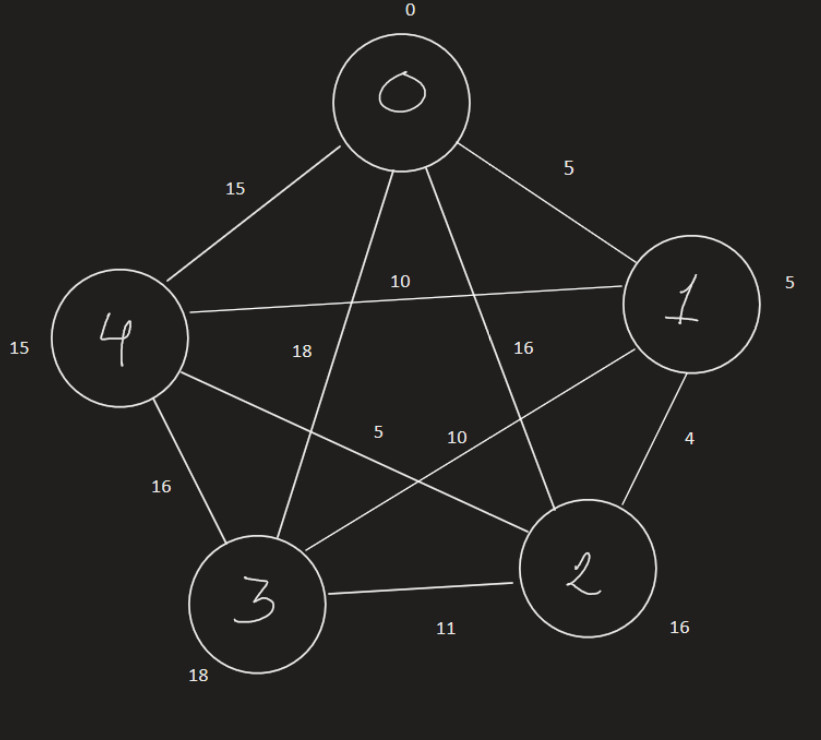
\includegraphics[scale = .5]{grafos1}
\caption{Grafo inicial}
\end{figure}

\begin{figure}[!htbp]
\centering
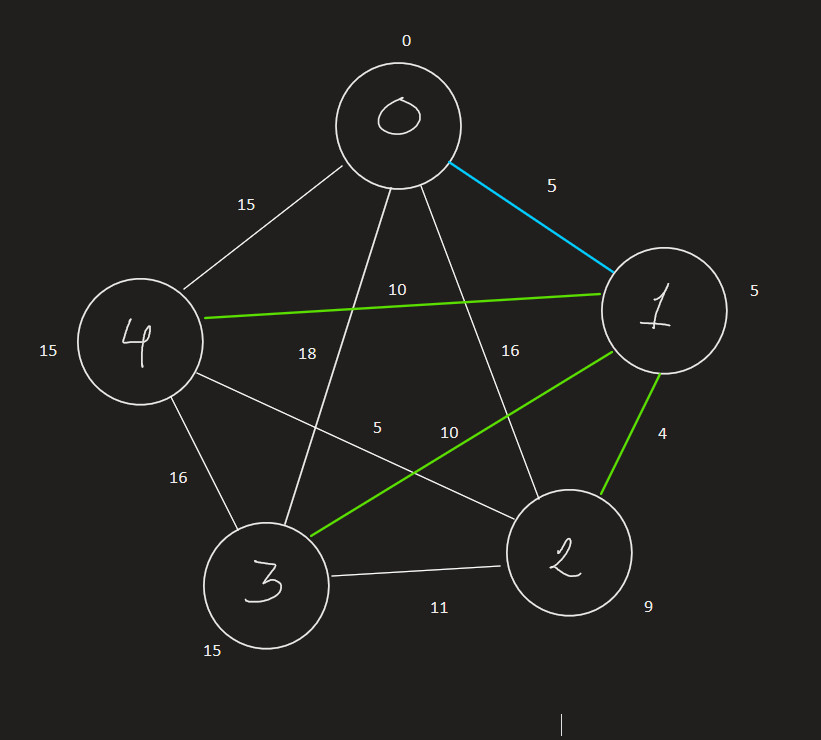
\includegraphics[scale = .5]{grafos2}
\caption{Primero se visita al nodo al nodo adyacente más cercano al origen.}
\end{figure}


\begin{figure}[!htbp]
\centering
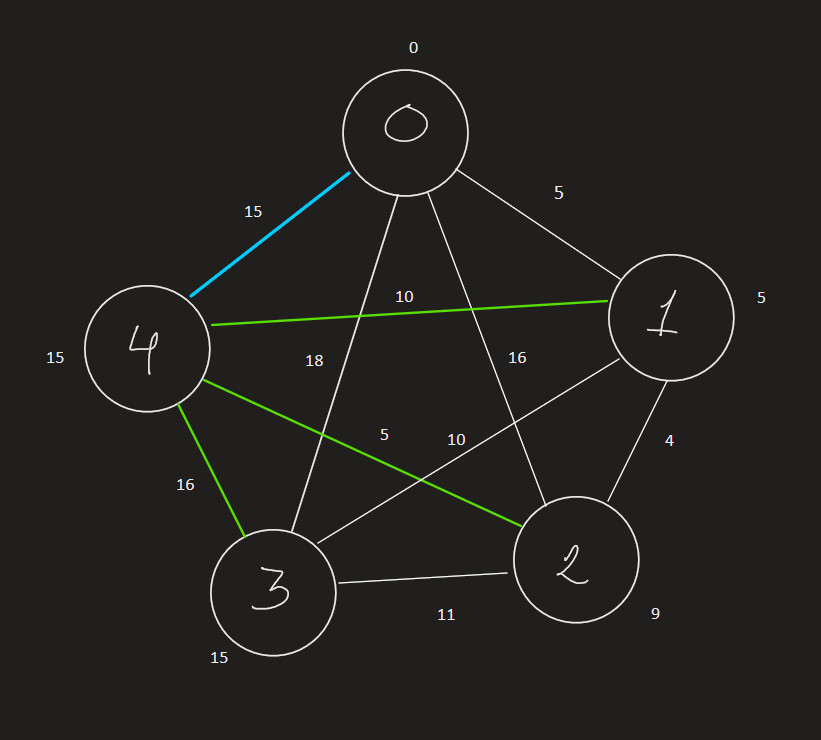
\includegraphics[scale = .5]{grafos3}
\caption{Después se visita el segundo más cerca.}
\end{figure}

\begin{figure}[!htbp]
\centering
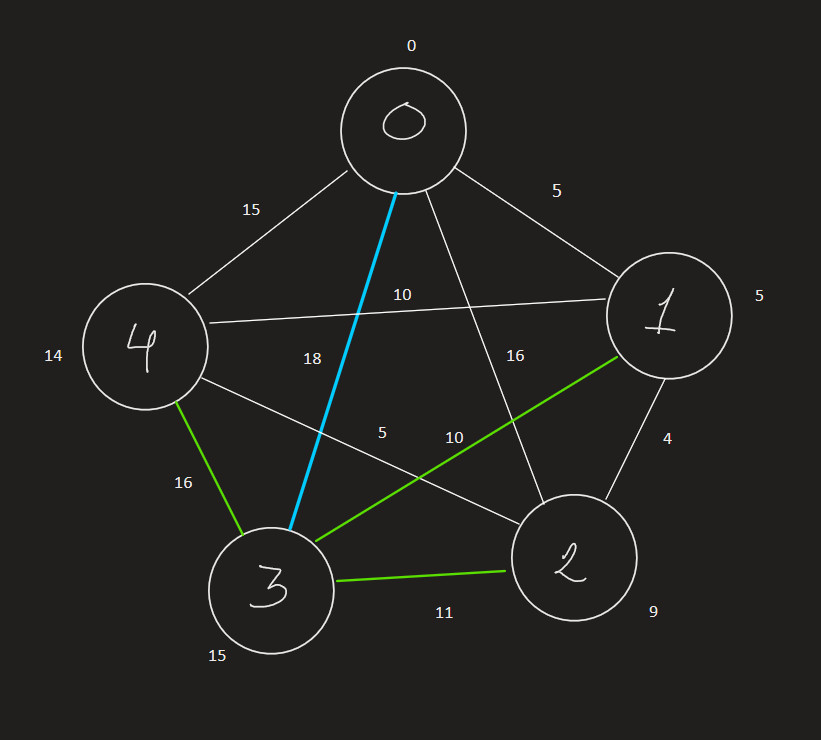
\includegraphics[scale = .5]{grafos5}
\caption{El algoritmo finaliza una vez que se visitó el más lejano.}
\end{figure}

\section{Paralelización del Algoritmo}
\subsection{Nivel de paralelismo}
Muchos algoritmos realizan cálculos atravesando iterativamente una gran estructura de datos por medio de un bucle. Por lo general, un bucle se ejecuta secuencialmente, lo que significa que los cálculos de la i-ésima iteración no se inician antes de que se completen todos los cálculos de la (i - 1) ésima iteración. Este esquema de ejecución se denomina ciclo secuencial.
\par
Si no hay dependencias entre las iteraciones de un bucle, las iteraciones se pueden ejecutar en un orden arbitrario y también se pueden ejecutar en paralelo por diferentes procesadores. Entonces, dicho bucle se denomina bucle paralelo.
\par 
En el caso del programa del Algoritmo de Dijkstra, cada hilo ejecuta una o más de las iteraciones, es decir, asume la responsabilidad de uno o más valores de i. Es por esto que podemos afirmar que el nivel de paralelismo que se maneja es a nivel de ciclo.

\subsection{Métricas de desempeño}
El principal propósito de escribir programas paralelos es aumentar el rendimiento con respecto a su contraparte secuencial. Para poder medir esto se establecieron las métricas de desempeño, que proporcionan elementos para decidir si los programas valen la pena o no.
\par
El tiempo de procesamiento del programa del Algoritmo de Dijkstra fue tomado en tres distintos procesadores con el mismo grafo para todos los casos. Los procesadores utilizados fueron los siguientes:
\par
Procesador 1: Intel i5, 2.50 GHz, 4 núcleos
\par
Procesador 2: Intel i5, 1.4 GHz, 4 núcleos
\par
Procesador 3: Intel i7, 2 GHz, 8 núcleos
\par
Los resultados obtenidos se muestran a continuación:

\begin{figure}[!htbp]
\centering
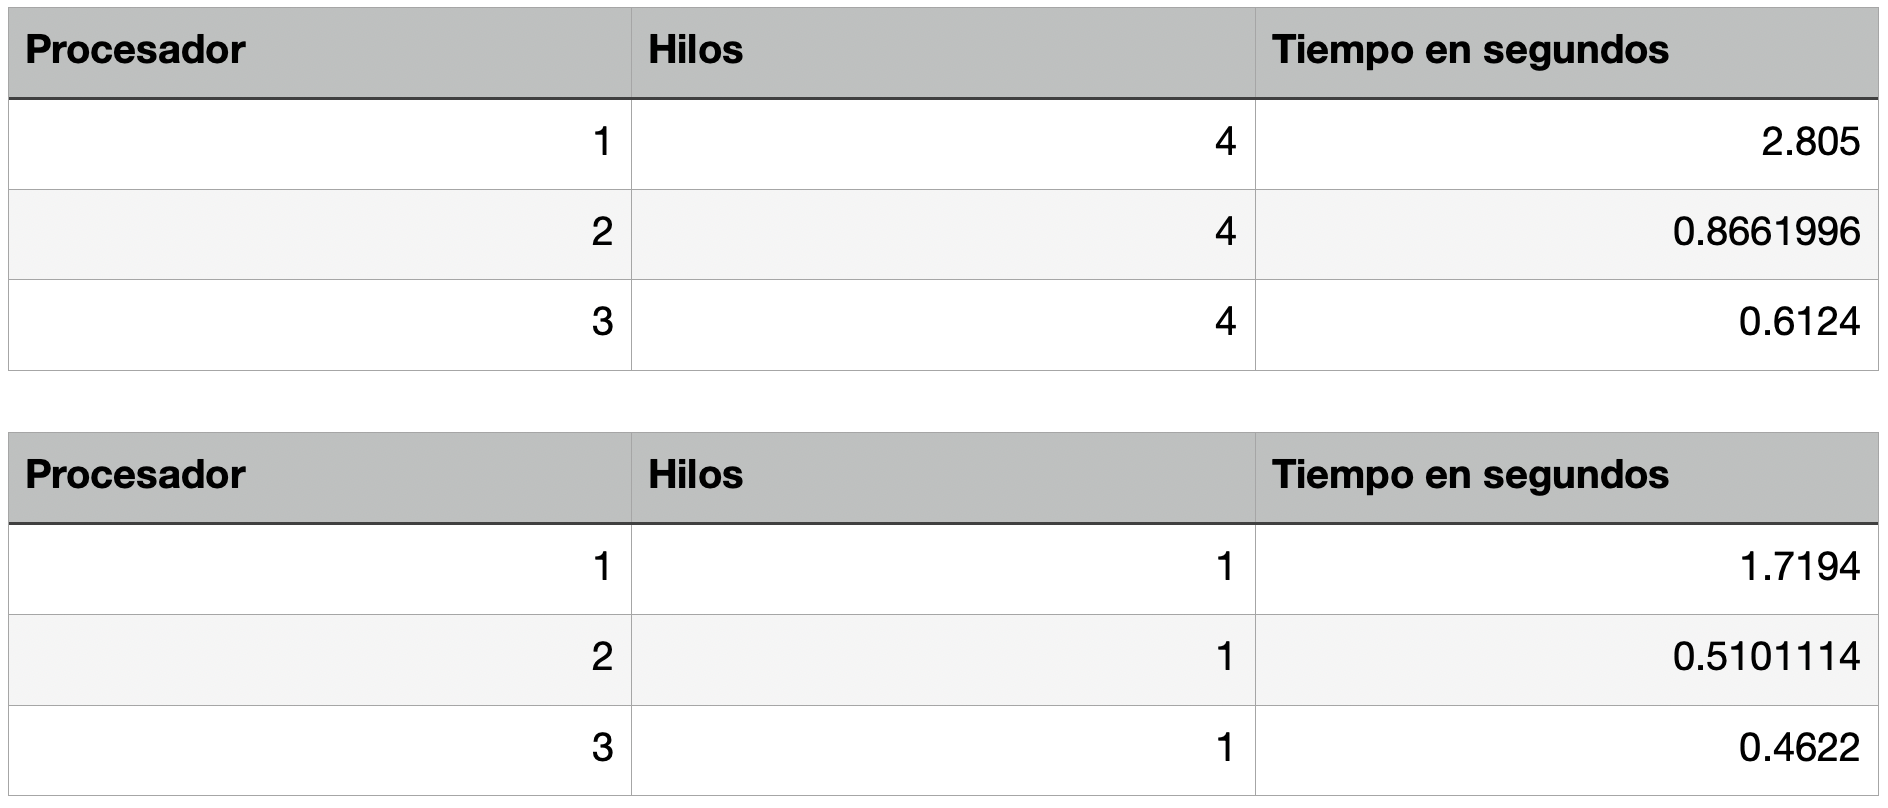
\includegraphics[scale = .5]{tiempo}
\caption{Para la toma del tiempo se utilizó la función omp\_get\_wtime() de la biblioteca omp.h}
\end{figure}

\subsubsection{Speedup}
Para el análisis de programas paralelos, una comparación con el tiempo de ejecución de una implementación secuencial es especialmente importante para ver el beneficio del paralelismo.
\par
El speedup de una implementación paralela expresa el ahorro de tiempo de ejecución que se puede obtener utilizando una ejecución paralela en n procesadores en comparación con la mejor implementación secuencial.
\par
Para el programa del Algoritmo de Dijkstra se obtuvo lo siguiente:

\begin{figure}[!htbp]
\centering
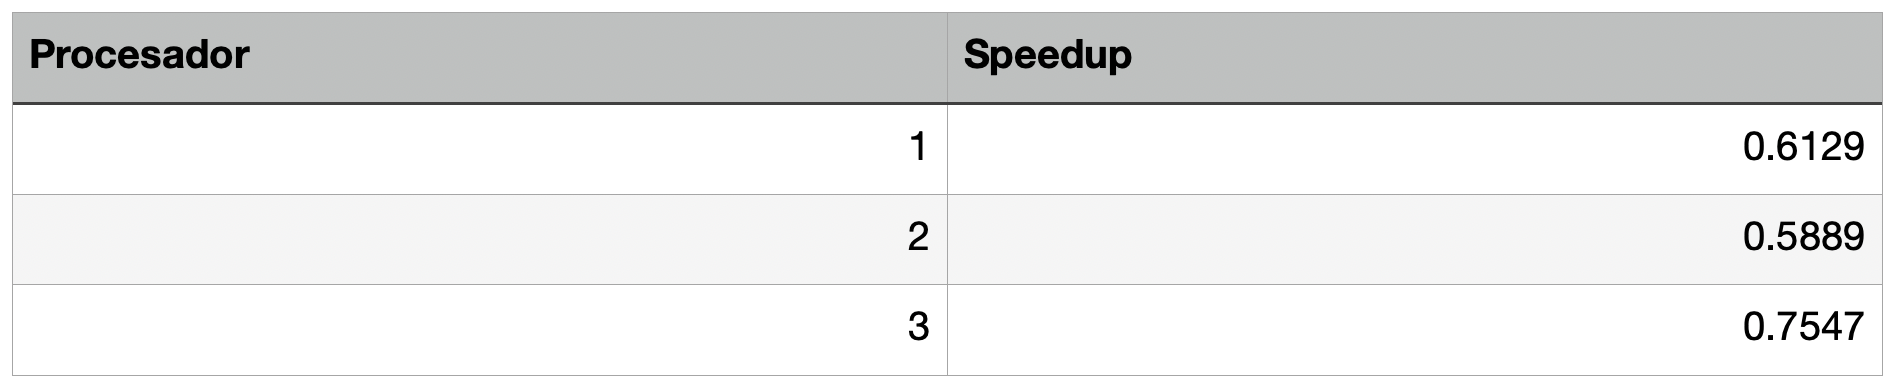
\includegraphics[scale = .5]{speedup}
\end{figure}

En los tres procesadores se observa que el valor del speedup es menor que la unidad. Esto quiere decir que el algoritmo ejecutado en forma paralela no presenta una mejora en cuanto al tiempo de ejecución, al contrario, hace que el programa se ejecute más lento.

\subsubsection{Eficiencia}
La eficiencia se define como la medida de la fracción de tiempo en la que cada procesador es usado para resolver el problema en cuestión de forma útil. En otras palabras, refleja el aprovechamiento de los recursos de hardware del sistema.
\par
Los cálculos de eficiencias obtenidos fueron los siguientes:

\begin{figure}[!htbp]
\centering
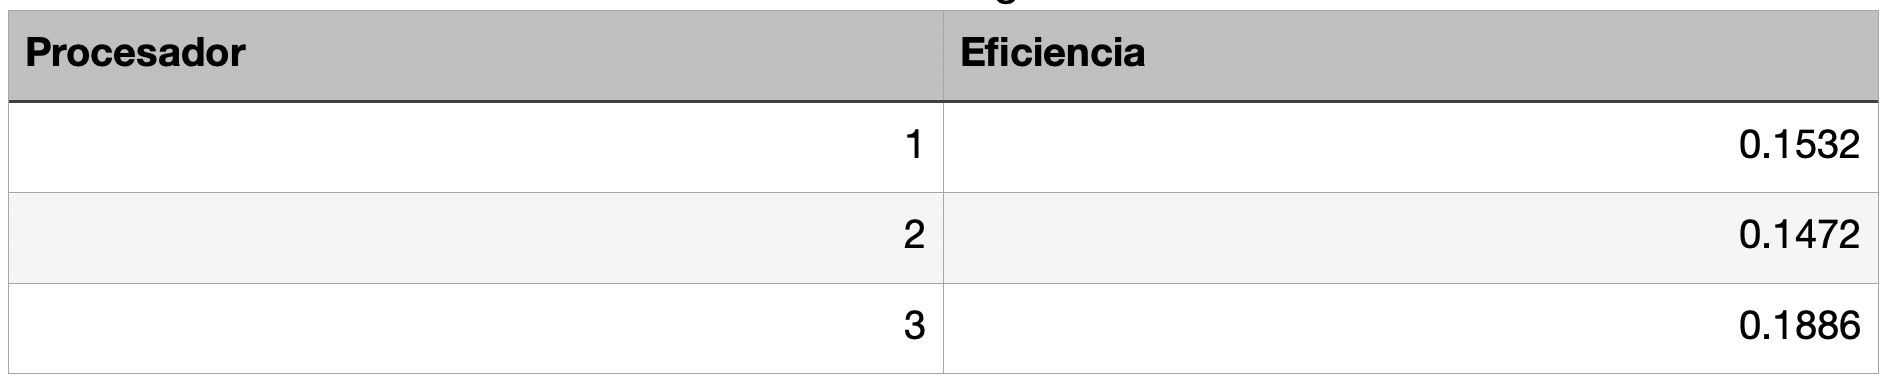
\includegraphics[scale = .5]{eficiencia}
\end{figure}

Si nuestros procesadores se utilizan de forma eficiente se espera que el tiempo de ejecución dedicado por cada procesador por el número de procesadores sea igual al tiempo de ejecución en un sólo procesador. Esto quiere decir que se requiere un valor cercano a la unidad. En base a los resultados obtenidos, se puede observar que están más cercanos a 0 que a 1, por lo que el programa no tiene una buena eficiencia.

\subsubsection{Fracción serial}
La fracción serial relaciona el speedup y la eficiencia con el propósito de tomar en cuenta otros factores además del tiempo.
\par
Los resultados se muestran a continuación:

\begin{figure}[!htbp]
\centering
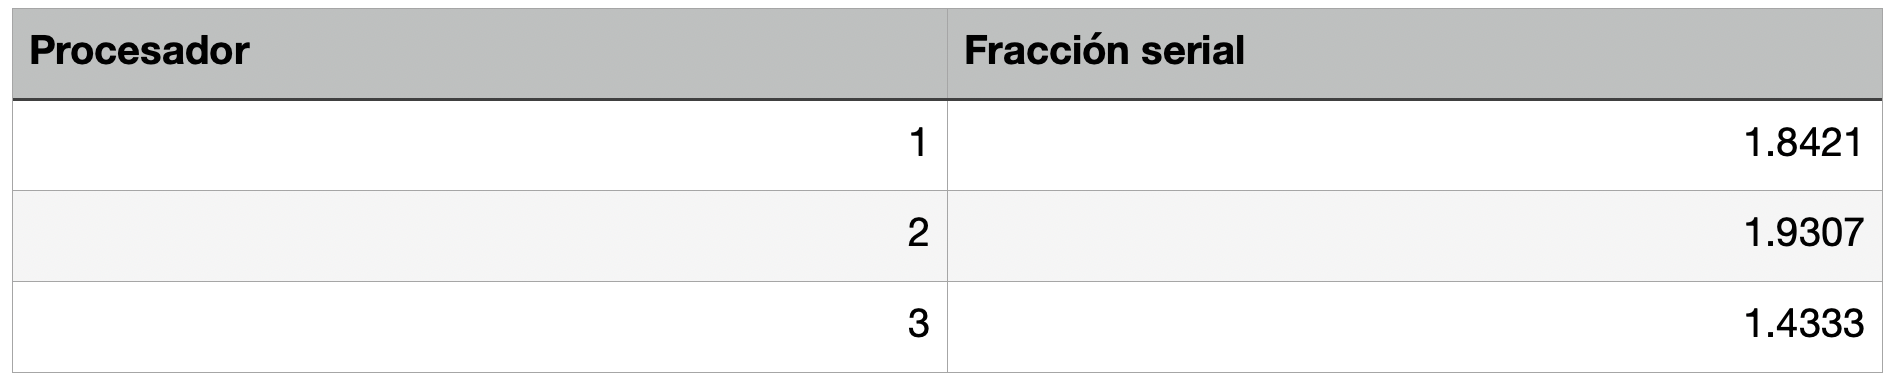
\includegraphics[scale = .5]{fraccion}
\end{figure}

Después de obtener las métricas de desempeño podemos afirmar que el programa no presenta una mejora en cuanto a su versión secuencial. En un apartado posterior se hará un análisis más profundo de esto.

\subsection{Formas de comunicación}
Una región paralela es ejecutada por varios hilos que acceden a los mismos datos compartidos, por lo que es necesaria la sincronización para proteger las regiones críticas o evitar la condición de carrera. OpenMP ofrece varios constructores que se pueden utilizar para la sincronización y coordinación de hilos dentro de una región paralela. El constructor critical especifica una región crítica que solo puede ser ejecutada por un único hilo a la vez. 
\par
Dentro del código del Algoritmo de Dijkstra encontramos distintas partes en donde se presentan regiones críticas, es por ello que se utiliza el constructor critical y otros constructores que ayudan a la sincronización de hilos como single y barrier.

\subsection{Granularidad}
El tiempo de cálculo de una tarea se denomina granularidad: las tareas con muchos cálculos tienen una granularidad de grano grueso, las tareas con solo unos pocos cálculos son de grano fino. 
\par
En el caso del programa del Algoritmo de Dijkstra se presenta una granularidad de tipo fina, ya que en cada región paralela hay pocas instrucciones. Lamentablemente, esto afecta directamente al desempeño del programa debido a que hay una gran sobrecarga de comunicación y sincronización de los hilos.

\end{document}